\documentclass[12pt, titlepage]{article}
\usepackage[ngerman]{babel}
\usepackage[utf8]{inputenc}
\usepackage{color}
\usepackage[a4paper, lmargin={3cm}, rmargin={2.5cm}, tmargin={3cm}, bmargin={2cm}]{geometry}
\usepackage{amssymb}
\usepackage{amsthm}
\usepackage{graphicx}
\usepackage{helvet}
\usepackage{microtype}
\usepackage{setspace}
\usepackage{csquotes}
\usepackage{xpatch}
\usepackage{comment}
\usepackage[backend=biber, %% Hilfsprogramm "biber" (statt "biblatex" oder "bibtex")
style=authoryear-ibid, %% Zitierstil (siehe Dokumentation)
natbib=true, %% Bereitstellen von natbib-kompatiblen Zitierkommandos
hyperref=false, %% hyperref-Paket verwenden, um Links zu erstellen
ibidpage=true
]{biblatex}
\addbibresource{literatur.bib}

\renewcommand{\familydefault}{\sfdefault}
\setlength\parindent{0pt}


\begin{document}
% Leere Titelseite
\pagenumbering{gobble}
\newpage\null\thispagestyle{empty}\newpage

\begin{titlepage}
    \normalsize{Hochschule Hannover, Fakultät IV: Wirtschaft und Informatik

    Bachelorarbeit im Studiengang Wirtschaftsinformatik, Wintersemester 2021/2022} 
    
    \sloppy 
    \textbf{\Large{\\Konzeption, Datenmodellierung und prototypischer Aufbau eines Prozess-Tracking-Tools zur Steuerung und Umsetzungsverfolgung einer S/4HANA Transformation im Vorgehensmodell eines IT-Beratungsunternehmens}}
    \vspace{10cm}
    \normalsize{\\Abgabedatum: 08. Februar 2022 \vspace{1cm}\\Lukas Hampel\\Matrikelnummer: 1481025\\Scharnhorststr. 8\\31785 Hameln\vspace{1cm}\\Erstprüfer: Herr Prof. Dr. Raymond Fleck\\Zweitprüfer: Herr Michael Bloß, adesso orange AG}
\end{titlepage}


\section*{Sperrvermerk}
Lorem
\newpage


\pagenumbering{Roman}
\setcounter{page}{3}
\section*{Vorbemerkung}

\newpage

\tableofcontents

\newpage

\section*{Glossar / Abkürzungsverzeichnis}

\newpage

\listoffigures{}
\listoftables{}

\newpage

\section*{Kurzfassung}

\newpage

\pagenumbering{arabic}
\setcounter{page}{1}
\begin{normalsize}
\linespread{1.5}

%Einleitung
\doublespacing
\section{Einleitung}
\subsection{Motivation}
Die SAP SE (fortan, in Abgrenzung zum Produkt, als \glqq{}die\grqq{} SAP bezeichnet) ist der größte Anbieter für Unternehmenssoftware in Europa und hat mit dem Produkt SAP-ERP eine der am weitesten verbreiteten Enterprise-Ressource-Planning (ERP)-Software geschaffen. \\Mit der neusten Generation SAP S/4HANA sollen in den nächsten Jahren die bereits etablierten Versionen SAP R/2 und SAP R/3 sukzessive abgelöst werden, bevor die Unterstützung, in Form von Weiterentwicklungen und Aktualisierungen, durch die SAP im Jahr 2030 vollständig eingestellt wird. Die Generation S/4HANA bringt viele neue Funktionen, unter anderem viele Cloud-Funktionalitäten mit sich, weshalb die Umstellung für die meisten Unternehmen eine große Hürde darstellt, die in der Regel nicht mit den intern vorhandenen Ressourcen bewältigt werden kann. Allerdings bringt die Aktualisierung auf die neuste Generation auch viele Chancen mit sich, um den Aufbau der Systeme und der darin abgebildeten Geschäftsprozesse komplett neu zu denken, 
%NICHT SCHÖN!!!!
da vieles bei der Umstellung sowieso angefasst werden muss. Das erleichtert bspw. die Trennung von historisch gewachsenen Strukturen und die Annäherung bzw. Etablierung des Industriestandards und dessen Best-Practises. Dadurch werden im Anschluss die Wartungskosten für die Systeme verringert und eine Optimierung und Effizienzsteigerung der Geschäftsprozesse erreicht.\\ Um eine solche Transformation durchzuführen, ist jedoch viel Wissen und Erfahrung im Projektmanagement und der Projektorganisation notwendig, vorallem aber auch viel Expertise in den Disziplinen der einzelnen Fachbereiche.
Die SAP setzt in den Bereichen Vertrieb, Service, Betrieb und  Entwicklung ihrer Produkte auf ein breit aufgestelltes Partnerprogramm, in dem Drittunternehmen aufgenommen werden können, um sich für eine Kooperation zu qualifizieren. Dadurch haben sich viele IT-Beratungsunternehmen auf das Themengebiet SAP spezialisiert und bieten nun auch eine SAP S/4HANA-Transformation für ihre Kunden an.

\subsection{Zielsetzung}
In der hier vorliegenden Bachelorarbeit aus dem Studiengang der Wirtschaftsinformatik soll es um die Konzeption, Datenmodellierung und den protypischen Aufbau eines Prozess-Tracking-Tools gehen, das im Vorgehensmodell eines IT-Beratungsunterneh- mens zur SAP S/4HANA-Transformation zum Einsatz kommen soll.\\ 
Das Tool soll auf dem gesamten Transformationspfad in einem S/4HANA-Projekt produktiv zum Einsatz kommen und frühzeitig einen 
Überblick über alle betroffene Transformationsobjekte wiedergeben. 
%nicht schön
Dadurch soll erreicht werden, dass zu jedem Zeitpunkt der aktuelle Fortschritt der Transformation im jeweiligen Prozess wiedergegeben werden kann und kein Artefakt außer acht gelassen wird, wodurch Probleme im späteren Projektverlauf vermieden werden sollen, indem stets alle Aspekte betrachtet werden können.



%Methodik
\section{Methodik und Vorgehen}
\subsection{Methodik}

\subsection{Vorgehen}
%Anfang nochmal ändern 
Dazu wird zunächst auf die einschlägigen Begrifflichkeiten eingegangen um sich dann dem Themenkomplex der S/4HANA-Transformation zu nähern und ihre Eigentschaften und Besonderheiten zu erklären. Im Anschluss wird zuerst das Unternehmen, in dessen Kontext sich diese Arbeit abspielt, vorgestellt, um dann genauer auf das Geschäftsmodell und das Vorgehensmodell zur S/4HANA Transformation einzugehen. \\
Danach wird der aktuelle Ist-Zustand des Tools, bzw. die Form, die momentan verwendet wird, vorgestellt und genauer darauf eingegangen, warum diese Form durch eine Neuentwicklung ersetzt werden sollte. Schließlich wird die Konzeption des Programms stattfinden. Dazu werden im ersten Schritt die Anforderungen analysiert, indem Interviews mit unterschiedlichen Key-Usern und Stakeholdern geführt werden, um daraus verschiedene Anwendungsfälle und -beispiele heraus zu filtern. In der Anforderungsanalyse werden sich ebenfalls Geschäftsprozessmodelldiagramme, erste Klassendiagramme und Sequenzdiagramme wiederfinden, um die Anforderungen an die Entwicklung zu visualisieren. Im nächsten Schritt werden die erarbeiteten Anforderungen ausgeprägt


%Grundlagen
\section{Grundlagen}
\subsection{ERP-Systeme}
ERP ist ein Akronym für den englischen Begriff \glqq{}Enterprise Ressource Planning\grqq{}, also das Planen von Unternehmensressourcen, u.a. in den Bereichen Beschaffung, Produktion, Vertrieb, Personalwirtschaft und Finanzwesen. \footcite[Vgl.][523]{wibuch} Ein ERP-System beschreibt somit eine Software, die Prozesse aus diesen Bereichen in einem Anwendungspaket integriert und die dabei anfallenden Daten in einer zentralen Datenbank abspeichert. Dadurch werden Redundanzen in der Datenhaltung vermieden und bereichsübergreifende Unternehmensprozesse ermöglicht \footcite[Vgl.][523]{wibuch}. ERP-Systeme nutzen in der Regel eine Client-Server-Architektur und sind komponentenorientiert, das heißt, sie können, je nach Anforderungen ihres Wertschöpfungsprozesses, ihre benötigten Komponenten frei wählen. Dadurch ist eine schrittweise Einführung der ERP-Software, über einen längeren Zeitraum, möglich. \footcite[Vgl.][524 f.]{wibuch}

\subsection{SAP}
\subsubsection{Die SAP SE}
Die SAP SE wurde im Jahr 1972 von fünf ehemaligen IBM-Mitarbeitern unter dem Namen \glqq{}\underline{S}ystem\underline{a}nalyse und \underline{P}rogrammentwicklung GbR\grqq{}\footcite[Vgl.][]{think-ing}  mit dem Ziel gegründet, eine Standardanwendungssoftware für die Echtzeitverarbeitung zu entwickeln.  Im Jahr 1973 wurde durch die SAP mit dem \glqq{}System RF\grqq{} das erste Produkt für die Finanzbuchhaltung vorgestellt, was den Grundstein für die erste SAP-Generation \glqq{}SAP R/1\grqq{} legen sollte. Durch die ständigen Weiterentwicklungen wurde das System stets erweitert und fand bei immer mehr Kunden anklang. 1976 wurde die Gesellschaft bürgerlichen Rechts aufeglöst und in eine GmbH überführt. Im selben Jahr wurde bereits mit nur 25 Mitarbeitern ein Umsatz von 3,81 Mio. DM erzielt. \footcite[Vgl.][]{sap-fruehejahre}\\Im Jahr 1979 folgt schließlich die zweite Produktgeneration \glqq{}SAP R/2\grqq{}

\subsubsection{SAP-ERP}

\subsubsection{SAP HANA}

\subsubsection{S/4HANA}

\subsection{Transformation}



\newpage
\section{Umfeld}
\subsection{Vorstellung des Unternehmens}
\subsection{Geschäftsmodell}
\subsubsection{Beispiel Kunde}
\subsection{Einordnung AAT / Notwendigkeit}
\subsection{Notwendigkeit}
\subsection{Aufbau}
\subsection{Phasen}
\subsection{Einordnung des BTT}


%Ist-Zustand
\section{Erhebung des Ist-Zustand}

\subsection{Was bietet das Tool bereits heute}
Zum jetzigen Zeitpunkt exisitiert der Business-Transformation-Tracker bereits in Form eines Excel-Spreadsheets. Dieses wird bereits in einigen Transformationsprojekten des betrachteten Unternehmens verwendet und unterstützt dadurch schon heute die Mitarbeiter in den Projekten. \\Das Tool dient dazu in einem S/4HANA Transformationsprojekt 
\subsection{Welche Verbesserungspotenziale gibt es}

\subsection{Warum verbessern?}

\subsection{Geplante Erweiterungen des Funktionsumfangs}

\subsection{Interviews mit Stakeholdern}

%Anforderungsermittlung
\section{Ermittlung der Anforderungen}
\subsection{Ermittlung der Stakeholder}
Bevor mit der Ermittlung der Anforderungen begonnen wird, müssen zuerst die Stakeholder identifiziert werden, die ein allgemeines Interesse an der zu entwicklenden Software, bzw. dem Tool haben. Dabei handelt es sich um Personen, die entweder von dem fertigen Produkt profitieren, oder die später das Produkt zu ihrer täglichen Arbeit einsetzen und daher ein Interesse am Funktionsumfang und der Benutzerfreundlichkeit haben. 

\subsubsection{Analyse der Stakeholder}
Im Falle des Business-Transformation-Trackers wurde folgende Stakeholder ermittelt:
\begin{itemize}
    \item[] \emph{Oberes Management:} Das obere Management des auftraggebenen Unternehmens ist der Auftraggeber für das Entwicklungsprojekt und hat daher besonderes Interesse in der erfolgreichen Fertigstellung des Projekts und der produktivsetzung der Software um somit Wertschöpfung zu generieren. Dazu kommt, dass das Ziel der Software die Unterstüzung der Mitarbeiter in den Projekten ist und sich durch den Einsatz eine Effizienzsteigerung und Qualitätsverbesserung erhofft wird. Dadurch besteht die Möglichkeit der Reputationssteigerung gegenüber potentiellen Kunden und somit einer gesteigerten Nachfrage im Vertrieb, was ebenfalls im besonderen Interesse des Managements liegt. In Persona tritt das obere Management im Entwicklungsprojekt als Bereichsleiter \glqq{}SAP Consulting and Development\grqq{} in Erscheinung.
    \item[] \emph{Mittleres Management:} Die Mitarbeiter des auftraggebenen Unternehmen im mittleren Management fungieren in der Regel in der Rolle eines Abteilungs- oder Projektleiters und haben daher ein besonderes Interesse an dem Funktionsumfang an der zu entwicklenen Software, da sie durch den Funktionsumfang direkt in den Projekten profitieren können. So profitieren sie beispielsweise von einer übersichtlichen Ansicht des gesamten Projekts und können durch Auswertungen besser das Projekt verwalten. Außerdem besitzen die Mitarbeiter des mittleren Managements ein Interesse darin, dass das Tool durch die Mitarbeiter verwendet wird, damit die darin geführten Daten stets auf dem aktuellen Stand sind. 
    \item[] \emph{Senior Consultants:} Senior Consultants sind erfahrene Mitarbeiter des auftraggebenen Unternehmens und arbeiten in der Regel als Projektleiter in kleineren Projekten oder als Teilprojektleiter in Projekten mit größerem Umfang. Sie haben ein großes Interesse im Funktionsumfang des BTT und sind auch sehr an der Übersichtlichkeit und Benutzerfreundlichkeit der grafischen Oberfläche interessiert, da sie, zusammen mit den Consultants, am intensivsten mit dem Programm arbeiten werden. Dabei stehen die Ziele der Datenkonsistenz und der generellen Verfügbarkeit des BTT im Vordergrund, damit eine reibungslose Arbeit ermöglicht wird.
    \item[] \emph{Consultants:} Die Consultants, bzw. Berater bilden den Kern der Mitarbeiterschaft des auftraggebenen Unternehmens und treten in der Regel als Projektmitarbeiter in Erscheinung. Sie bilden die größte Zielgruppe, da sie am häufigsten mit dem Programm arbeiten werden und dort den Großteil der Datenerfassung durchführen werden. Deshalb ist es vom besonderen Interesse, den Projektmitarbeitern die Arbeit mit dem Produkt möglichst einfach zu machen und besonders auf die Benutzerfreundlichkeit in der Entwicklung zu achten. Dazu kommt, das es wichtig ist, diese Stakeholdergruppe möglichst in die Entwicklung mit einzubeziehen, um Verbesserungsvorschläge und Ideen in die Anforderungen mit aufzunehmen. 
    \item[] \emph{Entwickler:} Die (SAP-)Entwickler des Auftraggebers spielen nur eine untergeordnete Rolle im Kontext des Business Transformation Tracker, da die Befüllung und Auswertung nicht in ihr Aufgabenfeld gehört. Denkbar sind dennoch Szenarien, in denen sie aufgefordert werden einzelne Einträge in dem Programm vorzunehmen, zu denen ihre Expertise benötigt wird. Auch besteht ein großes Interesse an Benutzerfreundlichkeit und Übersichtlichkeit, damit auch bei seltener Nutzung der Umgang mit dem Programm nicht schwer fällt.
    \item[] \emph{Kunden:} Weitere Stakeholder sind die Kunden des Auftraggebers, da diese ebenfalls Berührungspunkte mit dem Programm haben werden, wenn es Teil ihres Transformationsprojekts wird. Sie haben ein besonderes Interesse an der gesteigerten Effizienz und der gesteigerten Qualität ihrer Transformation, da dies für sie eingesparte Ressourcen in Form von weniger Projekttagen, weniger Aufwänden für die Transformation und geringere Wartungskosten im Anschluss durch die gesteigerte Qualität der Prozesse bedeutet. Dazu kommt, dass es dazu kommen kann, dass in größeren Projekten die Mitarbeiter des Kunden ebenfalls in direkten Kontakt mit dem BTT kommen, um bspw. bei der Erfassung der Prozesse zu unterstützen. Dadurch entsteht ein großes Interesse an der Übersichtlichkeit und der Benutzerfreundlichkeit, damit auch bei einmaliger Benutzung das gewünschte Resultat zustande kommt.
\end{itemize}

\subsubsection{Riskobewertung der Stakeholder}
Von den unterschiedlichen Stakeholdern gehen unterschiedliche Risiken im Bezug auf den Erfolg des Produkts aus. So gibt es auf der einen Seite ein unterschiedliches Konfliktpotential, das durch die unterschiedliche Mächtigkeit der Stakeholder, verschiedene Probleme im späteren Einsatz des Tools herbeiführen kann. So wäre es zum Beispiel denkbar, dass ein Consultant die Arbeit mit dem BTT verweigert, wenn seine persönlichen Anforderungen, in Form von Benutzerfreundlichkeit, außer Acht gelassen werden, oder, das ein Mitarbeiter des mittleren Managements, in Form eines Projektleiters, den Einsatz von Anfang an garnicht erst vorsieht, wenn er der Meinung ist, dass das Tool keinen Mehrwert bietet, wenn seine Anforderungen an das Programm, beispielsweise in Form von Verfügbarkeit und Zuverlässigkeit, nur unzulänglich erfüllt werden.
\begin{figure}[ht]
    \centering
    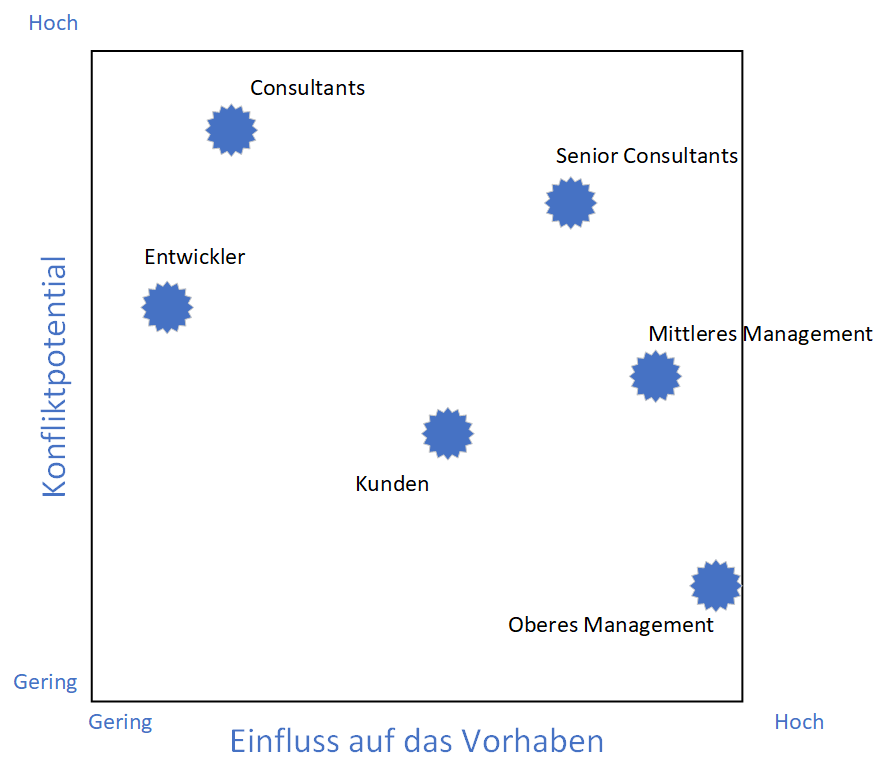
\includegraphics[scale=0.67]{Bilder/stakeholderRisiko.png}
    \caption[]{Subjektive Risikobewertung der genannten Stakeholder}
\end{figure}
Dieses Konfliktpotential lässt sich umgehen, indem die Personengruppen frühzeit in die Anforderungsermittlung mit eingebunden werden und sie dadurch, im Rahmen der Möglichkeiten, selbst bei der Produktentwicklung mitwirken können. Besonders bei Stakeholdern mit großer Macht und hohem Konfliktpotential ist es daher wichtig Maßnahmen zu definieren, wodurch dieses gesenkt werden kann.\footcite[Vgl.][S. 504 f.]{balzert}



\subsection{Erhebung der Anforderungen}
\subsubsection{Informationen durch den Auftraggeber}
Zur Ermittlung der Anforderungen fanden mehrere Gespräche mit dem Auftraggeber statt, in denen zum einen auf den aktuellen Ist-Zustand eingegangen wurde, aber auch Ideen und Umsetzungsvorschläge besprochen wurde. Diese Informationen wurden bereits in dem vorangegangenen Kapitel 5 in der Problemstellung und in der Beschreibung des Ist-Zustandes untergebracht und werden nun genutzt um daraus die Anforderungen an das in Auftrag gegebene Programm zu entwickeln. Während des Entwicklungsprozess besteht ein enger Kontakt zu dem Auftraggeber, wodurch auftretene Rückfragen schnell beantwortet werden können. 

\subsubsection{Befragung im Unternehmen}
Um von möglichst vielen Stakeholdern Anforderungen an eine Neuentwicklung des Business Transformation Trackers zu erhalten, wurde mit den Mitarbeitern des auftraggebenen Unternehmen, die bereits mit der aktuellen Umsetzung des BTT, bzw. seinem Vorgänger, gearbeitet haben, eine Onlinebefragung durchgeführt. Ziel der Befragung war es zum einen das generelle Meinungsbild der Mitarbeiter zu dem BTT zu erfassen und zum anderen mögliche Verbesserungsvorschläge und Ideen der Stakeholder aufzugreifen, um daraus Anfoderungen an einen Neuaufbau des BTT zu entwickeln. Die Umfrage richtet sich dabei an alle internen Stakeholder, das heißt an die Mitarbeiter des oberen und mittleren Mangements, an die Senior Consultants, Consultants und Entwickler. Dadurch soll ein möglichst breites Bild entstehen, dass alle Interessen abdeckt, sodass kein Stakeholder vernachlässigt wird.\\Die Umfrage wurde mit der Online-Plattform \glqq{}Microsoft Teams\grqq{} umgesetzt, das Bestandteil der im Unternehmen eingesetzen Softwaresuite \glqq{}Microsoft 365\grqq{} ist. Die Umfrage wurde anonym durchgeführt, mit der Möglichkeit am Ende freiwillig seine Kontaktdaten anzugeben, um Rückfragen zu den gegebenen Antworten und Vorschlägen zu ermöglichen. Der Fragenkatalog bestand aus drei Abschnitten, zuerst allgemeine Fragen zur Person und zur Position im Unternehmen, als nächstes mit Fragen zur Meinung über den BTT und zum Schluss mit der Möglichkeit Verbesserungsvorschläge und Ideen anzugeben. Um dem Betriebsklima im Unternehmen gerecht zu werden, wurde in der Umfrage auf die förmliche Anrede der Befragten verzichtet.

\subsubsection{Auswertung der Umfrage}

\subsection{Spezifikation der Anforderungen}
Im nun folgenden Unterkapitel werden die im letzten Kapitel, durch Onlinebefragung und in persönlichen Gesprächen, ermittelten Anforderungen spezifiziert, das heißt, systematisch ausgewertet. Es wird aufgrund einer nichtvorhandenen Ausschreibung des Projekts und des geringen Projektumfangs auf ein seperates Lasten- und Pflichtenheft verzichtet und stattdessen die Anforderungen in der hier beginnenden \glqq{}Requirements Specification\grqq{}, zu deutsch \glqq{}Anforderungsspezifikation\grqq{}, niedergeschrieben. Dazu wird sich an der von Helmut Balzert beschriebenen \glqq{}Schablone[n] für Lastenheft, Pflichtenheft und Glossar\grqq{}\footcite[S. 492]{balzert} orientiert. In dieser werden zuerst die Visionen und Ziele des Entwicklungsprojekt verfasst, danach die Rahmenbedingungen denen die Entwicklung unterliegt, im Anschluss der technische Kontext, in dem sich die Entwicklung abspielt und dann erst die funktionalen Anforderungen, die die Kernfunktionalität des Systems beschreiben gefolgt von den nichtfunktionalen Anforderungen, bzw. den Qualitätsanforderungen, in denen die messbare Qualität und das Verhalten des Systems beschrieben wird.\footcite[Vgl.][S. 492 ff.]{balzert}. Die Anforderungen sind natursprachlich verfasst und verfügen über einen einzigartigen Identifikator, um im späteren Verlauf auf sie verweisen zu können. Diese sind so aufgebaut, dass \glqq{} [j]ede Anforderung [..] mit einem Buchstaben [beginnt] [...], gefolgt von einer Zahl, eingschlossen in Schrägstriche. Der Anforderungstyp wird durch einen Buchstaben gekennzeichnet [...]. Am Anfang werden  die Zahlen in Zehnerschritten durchnummeriert, sodass spätere fachlich dazugehörige Anforderungen zwischgefügt werden können.\grqq{} \footcite[S. 493]{balzert}

\subsubsection{Visionen und Ziele}
Die hier aufgezählten Visionen und Ziele sind Ausdruck der mit dem fertigen Produkt zu erreichenden Zukunft. Visionen sind dabei abstrakter und generisch verfasst, Ziele konkretisieren diese dann im Anschluss.\footcite[Vgl.][S. 457]{balzert}
\begin{itemize}
    \item[] \emph{/V10/} Der Auftraggeber soll durch den Business Transformation Tracker eine Qualitätssteigerung und Effizienzverbesserung in seinen Transformationsprojekten erreichen.
    \item[] \emph{/V20/} Die Anwender sollen mit dem Business Transformation Tracker während des gesamten Projektzeitraums die in SAP umgesetzten Prozesse erfassen und nachverfolgen können.
    \item[] \emph{/V30/} In jedem adesso active transformation -Projekt soll der Business Transformation Tracker eingesetzt werden.
    \item[] \emph{/V40/} Das Produkt soll dem Anwender eine angenehme User Experience bieten und muss ihn in seiner Arbeit produktiv unterstützen.\\
\end{itemize}

\begin{itemize} 
    \item[] \emph{/Z10/} Der Business Transformation Tracker soll zu jedem Zeitpunkt den aktuellen Fortschritssgrad ausgeben können, um schnell eine Übersicht zu erhalten.
    \item[] \emph{/Z20/} Dem Anwender soll es möglich sein, unterschiedliche Projekt aufrufen zu können.
    \item[] \emph{/Z30/} Die Ziele der Informationssicherheit (Authentizität, Vertraulichkeit, Integrität) dürfen nicht verletzt werden.
    \item[] \emph{/Z40/} Alle bereits jetzt implementierten Funktionen werden in die Neuentwicklung übernommen.         
    \item[] \emph{/Z50/} Der Business Transformationen Tracker soll den Funktionsumfang der jetzigen Lösung überbieten.  
    \item[] \emph{/Z60/} Das Anlegen eines Projektes im BTT dauert nicht länger als eine Minute.
    \item[] \emph{/Z70/} Die Erstellung eines Prozesschrittes ist dem Benutzer intuitiv möglich.
    \item[] \emph{/Z80/} Die Anwendung ist auf den verbreitetsten Systemen, Windows, Mac und Linux, einsetzbar.
\end{itemize}

\subsubsection{Rahmenbedingungen}
Als Rahmenbedingungen bezeichnet man Einschränkungen, die in der Entwicklung der Software berücksichtigt werden müssen. Diese sind entweder technischer oder organisatorischer Natur.\footcite[Vgl.][S. 459 f.]{balzert}
\begin{itemize}
    \item[] \emph{/R10/}
    \item[] \emph{/R20/}
\end{itemize}

\subsubsection{Kontext und Überblick}
Der Kontext beschreibt die technische Umgebebung, in die die Entwicklung eingebettet ist und welche Abhängigkeiten und Schnittstellen zu anderen Systemen exisitieren.\footcite[Vgl.][S. 461 f.]{balzert} 
\begin{itemize}
    \item[] \emph{/K10/}
    \item[] \emph{/K20/}
\end{itemize}

\subsubsection{Funktionale Anforderungen}
Die Funktionalen Anforderungen beschreiben den Funktionsumfang des Systems. Sie werden auf oberster Abstraktionsebene beschrieben.\footcite[Vgl.][S. 496]{balzert} Folgende funktionale Anforderungen wurden erarbeitet:
\begin{itemize}
    \item[] \emph{/F10/}
    \item[] \emph{/F20/}
\end{itemize}

\subsubsection{Qualitätsanforderungen}
Die nichtfunktionalen Anforderungen, bzw. Qualitätsanforderungen spiegeln Eigenschaften wieder, die das gesamte System und somit alle funktionalen Anforderungen betreffen. Die Qualitätsanforderungen werden anhand unterschiedlicher Kriterien kategorisiert, der \textbf{F}unktionalität, der \textbf{Z}uverlässigkeit, der \textbf{B}enutzbarkeit, der \textbf{E}ffizienz, der \textbf{W}artbarkeit und der \textbf{P}ortabilität.\footcite[Vgl.][S. 494 f.]{balzert} Die ermittelten nichtfunktionalen Anforderungen lauten wie folgt:
\begin{itemize}
    \item[] \emph{/Q10/}
    \item[] \emph{/Q20/}
\end{itemize}


%Anforderungsanalyse
\section{Analyse der Anforderungen}
%überarbeiten, an neues Buch anpassen
%Anforderungen --> Anforderungsspezifikation --> Fachliche Lösung
In dem nun folgendem Kapitel wird die Anforderungsanalyse behandelt. Orientiert wird sich dazu an dem Vorgehensmodell von Helmut Balzert, das ausführlich in dem Modul BIS-134 Anforderungsanalyse des Studiengangs Wirtschaftsinformatik der Hochschule Hannover behandelt wurde.\\Die Anforderungsanalyse ist einer der ersten Schritte im Softwareentwicklungsprozess und hat zum Ziel die Anforderungen zu ermitteln, die das System, in diesem Fall der Business Transformation Tracker, leisten soll, sowie diese zu definieren. Dadurch soll eine größtmögliche Abdeckung der gestellten Anforderungen erreicht werden und Unstimmigkeiten mit dem Kunden, bzw. dem Auftraggeber, in Bezug auf Funktion und Umfang, vermieden werden. Im Wasserfallmodell nach Balzert ist die Anforderungsanalyse in der Definitionsphase verortert und arbeitet somit mit den Ergebnisobjekten der vorangegangenen Planungsphase. \footcite[Vgl.][S. 100 ff.]{balzert} Die Ergebnisse der Anforderungsanalyse werden dem anschließenden Kapitel, der Konzeption und somit der Entwurfsphase, als Basis dienen.\\
Im Rahmen dieser    Darstellung in UML


\subsection{Ermittlung der Anforderungen}
Im nachfolgendem Kapitel werden die Anforderungen an die Software, die sich aus der Problemstellung und Gesprächen mit dem Auftraggeber ergeben haben, genauer spezifiziert. Im Anschluss folgen dann die zusätzlichen Anforderungen, die sich aus der Umfrage ergeben haben.

\subsubsection{Nichtfunktionale Anforderungen}
%Anforderungen müssen systematisch gewonnen werden von Beteiligten und Betroffenen, sonstige quellen

\subsection{Spezifizierung der Anforderungen}
%Ermittelte Anforderungen müssen spezifiziert werden, unter Berücksichtigung von festgelegten Methoden, Richtlinien, etc.

\subsection{Analyse der Anforderungen}
%Spezifizierte Anforderungen müssen anhand von Richtlinien und Checklisten analysiert werden

\subsection{Modellierung der Anforderungen}
%analysierte und validierte Anforderungen bilden Ausgangspunkt für Modellierung der fachlichen Lösung

\subsection{Verifikation der Anforderungen}

\subsection{Wahl der Entwicklungsplattform}
warum java, nicht web, nicht abap, nicht etc..
bewertung der it sicherheit anhand bestimmter kriterien (datenschutz, zugriffssicherheit, bewahrung von geschäftsgeheimnissne), java weil protierung auf allen plattformen (windows, unix, macos) verfügbar

\subsection{Pflichtenheft}
Durch den Auftraggeber wurden folgende Anforderungen gestellt:

\subsection{Use-Cases}
Akteure des IT-Systems definieren
Mitarbeiter: Projektmitarbeiter, Projektleiter, Teilprojektleiter
Usecase 1:
Der Projektleiter möchte ein neues Projekt anlegen und die Mitarbeiter zuordnen

Usecase 2:
Der Teilprojektleiter öffnet ein vorhandenes Projekt und fügt erfasst die Prozesse und Subprozesse

Usecase 3:
Ein Projektmitarbeiter möchte den aktuellen Fortschritt in einem Subprozess erfassen.

\subsection{Umgebung}
\subsection{Schnittstellen}

%Methodik
\begin{comment}
    %Methodik
    --> Wasserfallmodell nach Helmut Balzert(1995), S.100 ff.

    Anwendungsfälle
    Geschäftsprozessdiagramm, Aktivitätsdiagramm (Folie 94)
    Anwendungsfalldiagramm, -schablone
    Klassendiagramme --> Beziehungen --> Detailliertes Klassendiagramme
    Attribute Spezifizieren (exemplarisch), Operationen
    Sequenzdiagramm

    Pflichtenheft (genaue spezifizierung) 
    Verfeinerung des Lastenheftes
    Verbale Beschreibung dessen, was das System leisten soll (Auftraggebersicht)
    Dient i. a. als vertragliche Beschreibung des Lieferumfangs
    Einstiegsdokument für alle, die das System später pflegen und warten sollen
    Grundlage für die Erstellung des Produkt-Modells

    Ziel
    •Präzise Festlegung, WAS das System leisten soll (aus Sicht des Auftraggebers)
    Anforderungsanalyse
    •Ermittlung und Beschreibung der Anforderungen des Auftraggebers an ein IT-System
    •Bestimmung dessen, WAS das System leisten soll
    •Erstellen eines logischen Modells
\end{comment}

\section{Fachliche Lösung}
%OOA-Modell, GUI-Konzept, Prototyp, evtl. Benutzerhandbuch

\newpage
\section{Datenmodellierung}
\subsection{Aufbau}
\subsection{Beschreibung }
\subsection{...}

\newpage
\section{Konzeption}

--> Ziel
•Präzise Festlegung, WIE das Fachkonzept softwaretechnisch umgesetzt werden soll
Entwurf der Software-Architektur
--> Verteilte Java Anwenung mit Java Client und Java Server, Zentrale Anwendung, Web-Anwendung
•Technische Grobstruktur des Systems
Entwurf der Anwendungs-Architektur
•Zerlegung des Gesamtsystems in fachlich zusammengehörige Teile

\subsection{Datenmodell}
\subsection{Klassen}
\subsection{Beziehungen}
\subsection{...}

\newpage
\section{Prototyp}
Beschreibung des Prototypen
Implementierungsphase
Ziel
•Realisierung des Systems in Form von Programmen
Programmierung
Testen
•einzelne Komponenten
•Gesamtsystem

\subsection{Aufbau}
\subsection{Beschreibung Funktionalität}
\subsection{Fehlende Feautures}

\newpage
\section{Diskussion}
\subsection{...}

\section{Reflexion}

\newpage
\section{Fazit}
\subsection{Messung der Zielerreichung}



\newpage
\section{Schlussteil}


\newpage
\section{Anhang}
\section{Quellenverzeichnis}
\printbibliography
\section{Index}
\section{Erklärung zur ordnungsgemäßen Erstellung}







\end{normalsize}


\end{document}